\documentclass[11pt]{article}

\usepackage{dsfont}
\usepackage{amssymb}
\usepackage{mathtools}
\usepackage{geometry}
\geometry{a4paper}
\usepackage[parfill]{parskip}
\usepackage{graphicx}
\usepackage{amssymb}
\usepackage{epstopdf}
\usepackage{listings}
\lstset{language = C++}
\usepackage{url}

\newcommand{\re}[1]{\ensuremath{\operatorname{Re}(#1)}}
\newcommand{\im}[1]{\ensuremath{\operatorname{Im}(#1)}}

\newcommand{\Vr}{\ensuremath{U}}
\newcommand{\Vi}{\ensuremath{W}}
\newcommand{\Ir}{\ensuremath{H}}
\newcommand{\Ii}{\ensuremath{K}}
\newcommand{\Sr}{\ensuremath{P}}
\newcommand{\Si}{\ensuremath{Q}}

\newcommand{\Id}{\mathds{1}}

\title{Power Flow Theory}
\author{Dan Gordon}
\date{}

\begin{document}
\maketitle

\section{Nomenclature}
\begin{align*}
V &= \Vr + jW = \text{complex voltage.} \\
I &= \Ir + j\Ii = \text{complex current.} \\
S &= P + jQ = \text{complex power.} \\
y &= g + jb = \text{complex admittance.} \\
Z &= R + jX = \text{complex impedance.} \\
Y &= G + jB = \text{nodal admittance matrix.} \\
y_{ik} &= \text{complex admittance along branch $ik$.} \\
Y_{ik} &= G_{ik} + jB_{ik} = \text{nodal admittance matrix element $i, k$.} \\
&= 
	\begin{cases}
		-y_{ik}&\text{if $i \ne k$} \\
		\sum_{l \ne k} y_{il}& \text{if $i = k$}
	\end{cases} \\
\theta_{i} &= \text{the voltage angle of bus $i$.} \\
\theta_{ik} &= \theta_i - \theta_k = \text{the voltage angle difference between busses $i$ and $k$.} \\
I_{\text{br},i} &= \text{complex current injection from branches at bus $i$.} \\
I_{\text{zip},i} &= \text{total complex current injection from load at bus $i$.} \\
I_{\text{gen},i} &= \text{complex current non-ZIP injection due to the voltage controlled generation at bus $i$.} \\
S_{\text{gen},i} &= \text{complex power non-ZIP injection due to the voltage controlled generation at bus $i$.} \\
S_{ci} &= \text{constant power injection ZIP component of load at bus $i$.} \\
I_{ci} &= \text{constant current injection ZIP component of load.} \\
y_{ci} &= \text{constant impedance ZIP component of load.} \\
\delta_{ik} &= \text{the Kronecker delta, $\delta_{ik} = 1$ if $i = k$, 0 otherwise.}
\end{align*}

\section{Problem description}
The network is represented as a graph, with the nodes being \emph{busses} and the arcs being \emph{branches}. Busses are considered points at which there is a single value of voltage $V$. \emph{Ground} is considered to have zero voltage and can be considered as a special implicit bus. 

Power/current flows into the busses via branches, and also in the form of current injections at busses. The relationship between power, current and voltage is $S = I^*V$, so we can interchangeably talk about power and current flow, since one can be transformed into the other. Also, the impedance of a flow is defined by Ohm's law $V = IZ$, or $I = VY$ where $Y = 1/Z$. We use the convention that all flows into/out of busses are specified as injections: that is, positive is power or current flowing into the bus and negative is power or current flowing out of the bus.

\emph{Loads} and \emph{generation} at a bus are current flows between ground and the bus.

Load injections from ground at a bus can often be modeled as:
\begin{align}
	I = I_c + \frac{S^*_c}{V^*}  + VY_c
\end{align}
This is the \emph{ZIP} model: constant current, impedance, and power components. This is a good model for many types of load, but could also model certain types of generation - e.g. fixed power generation. However, we will always refer to this kind of generation as a negative load.

Generators may apply some kind of additional voltage control on the bus. Normally, we consider two types of generator busses: slack or swing generators, where the total complex voltage is kept fixed by injecting variable $P$ or $Q$, and $PV$ or voltage-controlled busses, where the voltage magnitude $V$ and power $P$ are kept fixed while injecting a variable current\footnote{Note that the voltage angle is relative to the slack bus, and so is a non-local property of the network, hence it usually does not make sense to control it anywhere except at the slack bus.}. A bus without any voltage control is a PQ bus, where the injections are purely determined by the ZIP loads.

In summary, all busses may have a constant ZIP load associated with them. In theory, this ZIP load can correspond to generation, if the total $P$ injection from the ZIP is positive. There are three types of busses. For PQ busses, the power/current injection is just that of the ZIP, and $V$ is free to vary. For SL (slack/swing/infinite) busses, there is additional current injected to keep the complex voltage constant. For PV busses, there is additional current applied to keep the bus at a constant voltage magnitude $|V|$ and constant real power $P$.

\section{Power flow equations in current form}
Recall in what follows that we write all bus quantities as injections \emph{into} the bus. Thus a normal load will use quantities expressed as negative injections, while a generator will have positive injections.

The total current injection into bus $i$ is:
\begin{align}
I_i &= I_{\text{br}, i} + I_{\text{zip},i} + I_{\text{gen}, i} = 0\\
I_{\text{br},i} &= -\sum_{k=0}^NY_{ik}V_k \\
I_{\text{zip},i} &= \frac{S^*_{ci}}{V^*_i} + I_{ci} - y_{ci}V_i \\
I_{\text{gen},i} &= \frac{S^*_{\text{gen},i}}{V^*_i}
\end{align}
where $I_i$ is the total current injection to bus $i$, $I_{\text{br},i}$ is the injection from all connected branches, $I_{\text{zip},i}$ is the injection due to the ZIP loads, and $I_{\text{gen},i}$ is the non-ZIP injection due to the generators.
The total current is zero, due to Kirchoff's current conservation law. Thus,
\begin{align}
I_i &= \frac{S^*_{ci} + S^*_{\text{gen},i}}{V^*_i} + I_{ci} - y_{ci}V_i - \sum_{k=0}^NY_{ik}V_k = 0
\label{EQ_POWERFLOW_COMPLEX}
\end{align}
where, as before,
\begin{align}
	Y_{ik} &=
		\begin{cases}
			-y_{ik}&\text{if $i \ne k$} \\
			\sum_{l \ne k} y_{il}& \text{if $i = k$}
		\end{cases} \\
\end{align}


Real and imaginary components are:
\begin{align}
	\Ir_i &= \frac{(P_{ci} + P_{\text{gen},i})\Vr_i + (Q_{ci} + Q_{\text{gen},i})\Vi_i}{|V|^2_i} + \Ir_{ci} -g_{ci}\Vr_i + b_{ci}\Vi_i \notag \\
	&+ \sum_{k=0}^N\left(-G_{ik}\Vr_k + B_{ik}\Vi_k\right) = 0\\
	\Ii_i &= \frac{(P_{ci} + P_{\text{gen},i})\Vi_i - (Q_{ci} + Q_{\text{gen},i})\Vr_i}{|V|^2_i} + \Ii_{ci} -g_{ci}\Vi_i + b_{ci}\Vr_i \notag \\
	&+ \sum_{k=0}^N\left(-G_{ik}\Vi_k - B_{ik}\Vr_k\right) = 0
\end{align}
Note that in practice the $y_c$ dependent zip load is often absorbed into the diagonal elements of $Y$.

The possible unknowns are the generator power $S_{\text{gen}}$ and the voltages $V$.

\subsection{PQ busses}
For PQ busses, there is no additional (non-ZIP) generation, and hence $S_{\text{gen}}$ can be set to zero. The unknown variables are the components of $V$.
\subsection{Slack busses}
For SL busses, $V$ is constant and the power flow equations give an explicit expression for $S$. Thus, all quantities at slack busses can immediately be found and thus they are considered constants in any solver equations.
\subsection{PV busses}
For PV busses, the power flow equations also hold, with both components of $V$ being unknown as was the case for PQ busses. $Q_{\text{gen}}$ is an additional variable, and an extra constraint also applies:
\begin{align}
\Delta |V|^2 = \Vr^2 + \Vi^2 - V_\text{PV}^2 = 0
\label{EQ_POWERFLOW_PV_CONSTRAINT}
\end{align}
where $V_{\text{PV}}$ is the voltage magnitude setpoint for the PV bus.

\subsection{Newton-Raphson equations}
Considering PQ busses only for the moment, the unknowns are the real and imaginary parts of $V$, and these equations can be solved using the Newton-Raphson method. Letting the function to which we want to find the zero be $f = \{\Ir, \Ii\}$, the unknows be $x = \{\Vr, \Vi\}$, we wish to solve $f(x) = 0$. Using the Jacobian
\begin{align}
J_{ik}(x) = \frac{\partial f_i(x)}{\partial x_k}
\end{align}
the NR method calculates the update to $x$ at each iteration as the solution to the linear equations
\begin{align}
-f_{(n)} &= J(x_{(n)})(x_{(n+1)}-x_{(n)}) = J(x_{(n)})\Delta x_{(n,n+1)}
\label{EQ_NR}
\end{align}
The Jacobian elements for variables $V$ are given by:
\begin{align}
	\frac{\partial \Ir_i}{\partial \Vr_{k}} 
		&= \left[-\frac{2\Vr_k((P_{ck} + P_{\text{gen},k})\Vr_k + (Q_{ck} + Q_{\text{gen},k})\Vi_k)}{|V|_k^4} + \frac{(P_{ck} + P_{\text{gen},k})}{|V|_k^2} \right]\delta_{ik} \notag \\
		&- (G_{ik} + g_{ci}\delta_{ik}) \\
	\frac{\partial \Ir_i}{\partial \Vi_{k}} 
		&= \left[-\frac{2\Vi_k((P_{ck} + P_{\text{gen},k})\Vr_k + (Q_{ck} + Q_{\text{gen},k})\Vi_k)}{|V|_k^4} + \frac{(Q_{ck} + Q_{\text{gen},k})}{|V|_k^2} \right]\delta_{ik} \notag \\
		&+ (B_{ik} + b_{ci}\delta_{ik}) \\
	\frac{\partial \Ii_i}{\partial \Vr_{k}}
		&= \left[-\frac{2\Vr_k((P_{ck} + P_{\text{gen},k})\Vi_k - (Q_{ck} + Q_{\text{gen},k})\Vr_k)}{|V|_k^4} - \frac{(Q_{ck} + Q_{\text{gen},k})}{|V|_k^2} \right]\delta_{ik} \notag \\
		&- (B_{ik} + b_{ci}\delta_{ik}) \\
	\frac{\partial \Ii_i}{\partial \Vi_{k}}
		&= \left[-\frac{2\Vi_k((P_{ck} + P_{\text{gen},k})\Vi_k - (Q_{ck} + Q_{\text{gen},k})\Vr_k)}{|V|_k^4} + \frac{(P_{ck} + P_{\text{gen},k})}{|V|_k^2} \right] \delta_{ik} \notag \\
		&- (G_{ik} + g_{ci}\delta_{ik}) \\
\end{align}

\subsubsection{Treatment of the slack bus}
There are no variables associated with the slack bus. The voltage is constant, and the power can be found after the rest of the busses are solved.

\subsubsection{PV busses}
As explained earlier, $PV$ busses add an extra variable, $Q$. This adds the following non-zero elements to the Jacobian:
\begin{align}
\frac{\partial \Ir_k}{\partial Q_{\text{gen},k}} &= \frac{\Vi_k}{|V|_k^2} \\
\frac{\partial \Ii_k}{\partial Q_{\text{gen},k}} &= -\frac{\Vr_k}{|V|_k^2}
\end{align}
They also add an extra constraint, Eq. (\ref{EQ_POWERFLOW_PV_CONSTRAINT}), reproduced here:
\begin{align}
\Delta |V|^2 = \Vr^2 + \Vi^2 - V_\text{PV}^2 = 0
\label{EQ_POWERFLOW_PV_CONSTRAINT_AGAIN}
\end{align}
with corresponding elements in the Jacobian being:
\begin{align}
\frac{\partial \Delta|V|^2_k}{\partial \Vr_k} &= 2 \Vr_k \notag
\frac{\partial \Delta|V|^2_k}{\partial \Vi_k} &= 2 \Vi_k
\label{EQ_PV_JAC_Q}
\end{align}
The NR update corresponding to this constraint row is:
\begin{align}
	-\Vr_k^2 - \Vi_k^2 + V_{\text{PV},k}^2 &= 2\Vr_k\Delta\Vr_k + 2\Vi_k\Delta\Vi_k
\end{align}
which gives
\begin{align}
\Delta \Vr_k &= \frac{V^2_{\text{PV},k} - \Vr_k^2 - \Vi_k^2- 2\Vi_k\Delta \Vi_k}{2\Vr_k}
\end{align}

Using these expressions, $\Delta \Vr$ may be eliminated from the NR equations for the PV bus. First write the Jacobian as if all busses were PQ. Let $k$ be any PV bus. Take the column corresponding to $\Delta \Vr_k$, and add its product with $-\Vi_k/\Vr_k$ to the matching column for  $\Delta \Vi_k$. Add its product with $(|V|^2_{\text{PV},k} - \Vr_k^2 - \Vi_k^2)/(2\Vr_k)$ to $f$ in Eq. (\ref{EQ_NR}). The column and the corresponding element of $x$ for $\Delta \Vr_k$ will now be replaced with a column and elment for $\Delta Q_{\text{gen},k}$. Set the column to zero, and then set the block diagonal elements, using Eq. (\ref{PV_JAC_Q}). Reinterpret the corresponding element of $\Delta x$ in Eq. (\ref{EQ_NR}) as now corresponding to $\Delta Q_{\text{gen},k}$ instead of $\Delta \Vr_k$.

\section{Formalism for modelling branches}
We have seen that branches can be modelled in the nodal admittance matrix formalism. For a network of lines of fixed impedance between the nodes, the  $2 \times 2$ nodal admittance matrix elements connecting any two nodes have the following form:
\begin{align}
	Y_{ik} &= 
		\begin{cases}
			-y_{ik}&\text{if $i \ne k$} \\
			\sum_{l \ne k} y_{il}& \text{if $i = k$}
		\end{cases}
\end{align}
where $y_{ik}$ describes a symmetric matrix with zeros on the diagonal.

What about a more general $Y$? If we make no assumptions about the elements of $Y$, then $I = -YV$ simply expresses the most general linear relationship between the voltage at a series of nodes and the current flowing into those nodes, assuming that all lines through which current can flow are passive (constant admittances).

How can we parse this relationship in terms of equivalent circuits? There is no single way. Note, however, that we can write, for a single phase branch, the following general decomposition of $Y$:
\begin{align}
	Y &= \left[
		\begin{array}{ll}
			a + b & -a \\
			-a + c & a + d
		\end{array}
	\right] \notag \\
	&= \left[
		\begin{array}{cc}
			a + b & -a \\
			-a & a + d
		\end{array}
	\right] +
	\left[
		\begin{array}{cc}
			0 & - \\
			- & a
		\end{array}
	\right]
\end{align}

wher
\begin{align}
Y_{s,ii} &= Y_{ii} + \sum_{k \ne i} Y_{ik} \notag \\
Y_{+,ij} &= \frac{1}{2}(Y_{ij} + Y_{ji}) \notag \\
Y_{-,ij} &= \frac{1}{2}(Y_{ij} - Y_{ji}) \\
\end{align}

Firstly, suppose that
\begin{align}
	Y_{ii} = \sum_{l \ne i} y_{il} + c, \hspace{3em} c \ne 0.
\end{align}
Then we see, from Eq. (\ref{EQ_POWERFLOW_COMPLEX}), that c is just the constant admittance component of a ZIP load, or, in other words, the shunt admittance to earth.

Secondly, suppose $Y$ is not symmetric. Then, effectively, there will be extra current flowing into one node that does not come from the other node. Let's split 

\section{Multi phase lines}
Lines are typically handled in terms of $a$, $b$, $c$ and $d$ matrices. Assume for discussion that there are three phases, so these are $3 \times 3$ matrices, and $V$ and $I$ are assumed to be 3-vectors.
\begin{align}
	\begin{bmatrix} V_0 \\ I_0 \end{bmatrix} &=
	\begin{bmatrix} a & -b \\ c & -d \end{bmatrix} \begin{bmatrix} V_1 \\ I_1 \end{bmatrix}
\end{align}
Be careful of signs! Conventionally, the equations are written in terms of currents entering and leaving the line. But we'll move to a nodal admittance model, and hence all currents are treated as injections. This is why we have a negative sign on $b$ and $d$.

These equations can be transformed to the following:
\begin{align}
	\begin{bmatrix} I_0 \\ I_1 \end{bmatrix} &=
	\begin{bmatrix} db^{-1} & c - db^{-1}a \\ -b^{-1} & b^{-1}a \end{bmatrix} \begin{bmatrix} V_0 \\ V_1 \end{bmatrix} = Y\begin{bmatrix} V_0 \\ V_1 \end{bmatrix} 
\end{align}
which defines the nodal admittance matrix $Y$.

What is the interpretation of $a$, $b$, $c$, $d$? From Kersting \cite{KerstingXXXXa}, using a pi-model of a transmission line, $Z$ being the matrix of self and cross impedances of the line, $\Id$ being the identity matrix and $Y_s/2$ being the shunt admittance matrix for each of the two legs of the pi, we have
\begin{align}
a = d &= \Id + \frac{1}{2}ZY_s \\
b &= Z \\
c &= Y_s + \frac{1}{4}Y_s Z Y_s
\end{align}
and thus
\begin{align}
Y &= \begin{bmatrix} Z^{-1} + \frac{1}{2}ZY_sZ^{-1} & \frac{1}{2}Y_s + \frac{1}{2}Y_sZY_s - Z^{-1}-\frac{1}{2}ZY_sZ^{-1}-\frac{1}{4}ZY^2 \\
-Z^{-1} & Z^{-1}+\frac{1}{2}Y \end{bmatrix} 
\end{align}
\subsection{Short three wire lines}
For three phase delta lines of up to around 80 km in length, the shunt admittance $Y_s$ is small enough to neglect, and thus the nodal admittance matrix is:
\begin{align}
	Y &=
	\begin{bmatrix} Z^{-1} & -Z^{-1} \\ -Z^{-1} & Z^{-1} \end{bmatrix}
\end{align}
which is very reminiscent of the expression used in the single wire definition of nodal admittance.
\section{Transformers}
\subsection{Single phase transformers}
For an ideal transformer with a single turns ratio $r = n_0/n_1$, we have
\begin{align}
\begin{bmatrix}V_0 \\ I_0\end{bmatrix} &= \begin{bmatrix}n & 0 \\ 0 & 1/n\end{bmatrix}\begin{bmatrix}V_1 \\ I_1 \end{bmatrix}
\end{align}
This can't be modelled correctly in the formalism of nodal admittance\footnote{in the same way that constant current and constant power injections can't be included in the nodal admittance matrix: they require separate terms in the powerflow equations.}: it does not describe a linear relationship between nodal currents and voltages, but rather a constraint between the voltages and a constraint between the currents. Two equaivalent circuits for an ideal transformer are shown in Fig. \ref{FIG_IDEAL_TRANS_EQUIV}.
\begin{figure}[!h]
	\begin{center}
		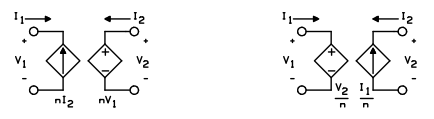
\includegraphics[width=(\textwidth-2cm)]{ideal_transformer_equiv.png}
	\end{center}
	\caption{
		Two equivalent circuits for an ideal transformer.
	}
	\label{FIG_IDEAL_TRANS_EQUIV}
\end{figure}
The relationships can be included in the powerflow equations specially, but more commonly real transformers are used, as described below; these may be expressed in the nodal admittance formalism.

A real transformer includes a leakage impedance (due to finite resistance of copper windings and core losses) and a shunt magnetising impedance. The latter is often large and may often be ignored. The nodal admittance matrix may be then derived:
\begin{align}
\begin{bmatrix}I_A \\ I_B \end{bmatrix} &= 
\begin{bmatrix}y_l/|a|^2 & -y_l/a^* \\ -y_l/a & y_l\end{bmatrix}
\begin{bmatrix}V_P \\ V_S \end{bmatrix}
\end{align}
where $a = V_P / V_S = N_P / N_S$ for an ideal transformer.

\subsection{Three-phase transformers}
The nodal admittance matrices of three-phase transformers may be derived from the single-phase expression, above, combined with information about the connections between phases.
\subsubsection{Delta-GWye}
\begin{figure}
\begin{center}
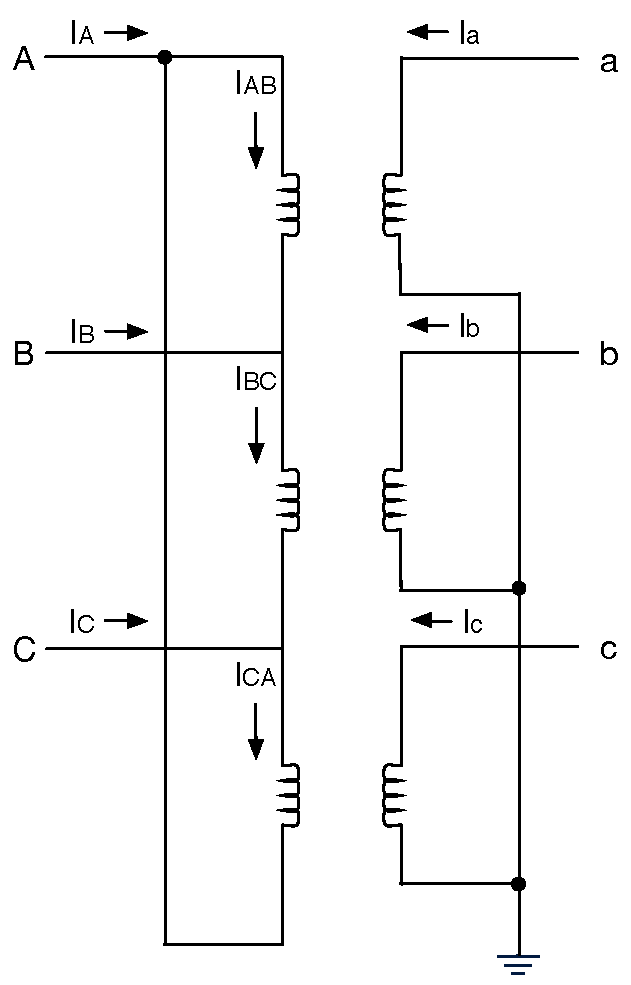
\includegraphics[width=7cm]{DeltaGWye.pdf}
\caption{Schematic of a Delta-GWye transformer}
\label{FIG_DELTA_GWYE}
\end{center}
\end{figure}
Considering Fig. \ref{FIG_DELTA_GWYE}, we have,
\begin{align}
I_{AB} &= \frac{y_l}{|a|^2}(V_A - V_B) - \frac{y_l}{a^*}V_a \\
I_{BC} &= \frac{y_l}{|a|^2}(V_B - V_C) - \frac{y_l}{a^*}V_b \\
I_{CA} &= \frac{y_l}{|a|^2}(V_C - V_A) - \frac{y_l}{a^*}V_c \\
I_a &= -\frac{y_l}{a}(V_A - V_B) + y_l V_a \\
I_b &= -\frac{y_l}{a}(V_B - V_C) + y_l V_b \\
I_c &= -\frac{y_l}{a}(V_C - V_A) + y_l V_c \\
\end{align}
Also, by the KCL, we have
\begin{align}
I_A &= I_{AB} - I_{CA} \\
&= \frac{y_l}{|a|^2}(2V_A - V_B - V_C) + \frac{y_l}{a^*}(V_c - V_a) \\
I_B &= I_{BC} - I_{AB} \\
&= \frac{y_l}{|a|^2}(2V_B - V_C - V_A) + \frac{y_l}{a^*}(V_a - V_b) \\
I_C &= I_{CA} - I_{BC} \\
&= \frac{y_l}{|a|^2}(2V_C - V_A - V_B) + \frac{y_l}{a^*}(V_b - V_c)
\end{align}
So we can immediately write down the nodal admittance relationship:
\begin{align}
\begin{bmatrix}I_A \\ I_B \\ I_C \\ I_a \\ I_b \\ I_c\end{bmatrix} &=
y_l \begin{bmatrix}
	2/|a|^2 & -1/|a|^2 & -1/|a|^2 & -1/a^* & 0 & 1/a^* \\
	-1/|a|^2 & 2/|a|^2 &  -1/|a|^2 & 1/a^*  & -1/a^* & 0 \\
	-1/|a|^2 &  -1/|a|^2 & 2/|a|^2 & 0 & 1/a^*  & -1/a^* \\
	-1/a & 1/a & 0 & 1 & 0 & 0 \\
	0 & -1/a & 1/a & 0 & 1 & 0 \\
	1/a & 0 & -1/a & 0 & 0 & 1
\end{bmatrix}
\begin{bmatrix}V_A \\ V_B \\ V_C \\ V_a \\ V_b \\ V_c\end{bmatrix}
\end{align}
with the nodal admittance matrix being specified by the matrix on the right, including the factor of $y_l$.
\section{The per-unit system}
Each bus has its own base voltage (usually expressed as Kv base). Bus voltages are then expressed in units of this voltage.

There is a single MVA base power defined for the entire network. Power is expressed in units of this power.

Current is expressed in units of $I_\text{base} = 
\end{document}